\section{Resultados}
\label{sec:results}

\begin{figure*}
    %\vspace{-4em}
    \centering
    \subfigure[QoE]{
    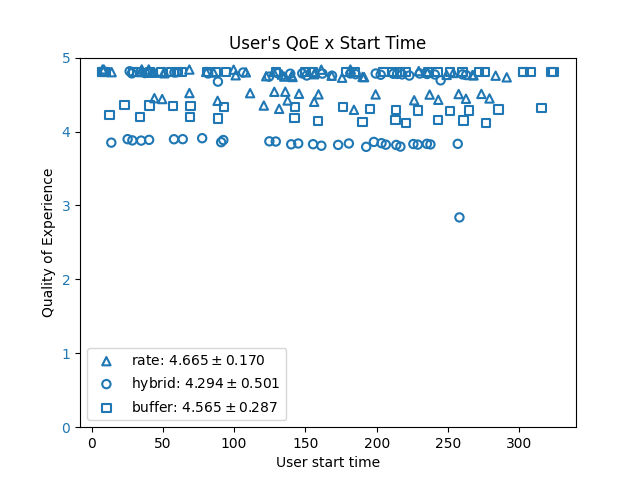
\includegraphics[width=0.32\linewidth]{charts/m_qoe_user.png}
    \label{fig:global-qoe-user}
    }
    \subfigure[HAS comparison]{
    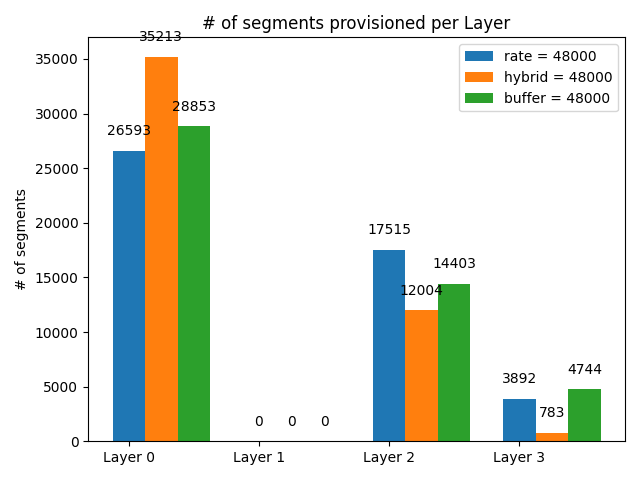
\includegraphics[width=0.3\linewidth]{charts/m_segments_per_layer_bu.png}
    \label{fig:plr-comparison-3}
    }
    \subfigure[Algorithm comparison]{
    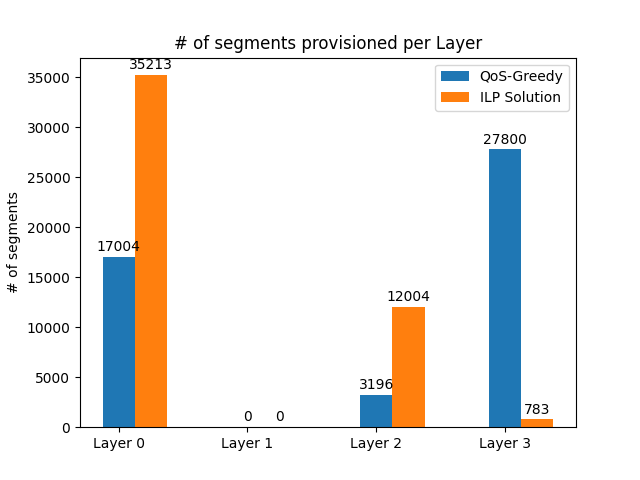
\includegraphics[width=0.32\linewidth]{charts/m_segments_per_layer_comp.png}
    \label{fig:plr-comparison-3}
    }
    \caption{Impact in a scenario (wall on the middle).
    }
    \label{fig:comparison-rof-3}
\end{figure*}


A Figura~\ref{fig:global-qoe-user} mostra o QoE global de cada usuário representada pode cada \textit{tick}, três algoritmos HAS são analisados com a solução ILP orquestrando a distribuição de video dentro da rede. Quando olhamos a media do desempenho sobre a perspectiva dos algoritmos HAS sendo executados pelo cliente, as heuristicas \textit{hydrid} e \textit{rate} tiveram um resultado melhor que o \textit{buffer}. O \textit{rate} teve uma leve oscilação entre os usuários, contudo os player sempre estiveram operando em boa qualidade, sem impactar diretamente o QoE e deixarem os usuários cairem no \textit{score}.

%Quando paramos para analisar a distribuição de requisições entre os níveis. 

Os experimentos ilustrados nas Figuras 4, 5 e 6 mostram a QoE média calculada pela Equação 2 quando há 15, 20 e 25 usuários por ponto de acesso solicitando vídeos na infraestrutura simulada. Cada boxplot representa os cenários somente nuvem, cache de borda e mobilidade. O desempenho médio geral do cache de borda é melhor do que os cenários somente nuvem e mobilidade, principalmente devido às escolhas de nós nos nós de peering de borda para atender às solicitações dos usuários. Por exemplo, no experimento Edge cache, quando ocorre congestionamento em links intermediários e 0,1 e e 0,2 , os nós de peering de borda são ativados para atender os usuários finais abaixo desses nós. Dessa forma, o tráfego que passa pelo link ascendente agora será suavizado, para que os usuários possam ter sua QoE aprimorada a um nível excelente. Como os usuários solicitam segmentos dos nós mais próximos e sem enlace de congestionamento em cenários com Edge cache, como esperado, observamos um aumento de QoE. A diferença de desempenho dos cenários somente na nuvem e de mobilidade para o experimento de cache de borda está próxima de um nível de satisfação para 15 e 20 usuários e aproximadamente dois níveis de satisfação para 25 usuários

Uma discussão interessante ocorre quando a QoE por usuário é analisada separadamente. De acordo com os resultados numéricos, a QoE final tende a piorar à medida que o número de usuários ativos aumenta. No entanto, isso não é totalmente verdade para o cenário de cache de borda, em que o QoE final para cada usuário permanece próximo. O desvio padrão de 0,037, 0,162 e 0,273, respectivamente, para cenários com 15, 20 e 25 usuários por AP, indica uma QoE mais próxima entre os usuários. Apenas no cenário de 25 usuários por AP, a QoE média apresentou queda com satisfação próxima da regular. Em contraste com os outros dois cenários apresentando uma satisfação dos usuários de boa a excelente. Enquanto para cenários de mobilidade e somente nuvem, a rede opera com um alto desvio padrão. À medida que o número de usuários aumenta, alguns outliers começam a aparecer com o pior nível de satisfação, ficando entre ruim e inadequado.

Com base nessas observações, uma estratégia simples de mover o vídeo para a borda pode melhorar significativamente a QoE do usuário. Desta forma, o sistema de transmissão de vídeo pode proporcionar qualidades de satisfação ao usuário e mantê-lo assistindo o vídeo até o final. No entanto, se não houver um gerenciamento correto das conexões em tempo real e um mecanismo dinâmico para lidar com uma carga variável proveniente, por exemplo, da mobilidade dos usuários, podemos concluir que o impacto introduzido pelas alterações do AP pode diminuir significativamente sua QoE. A experiência do usuário pode acabar piorando mesmo usando a borda da rede. O gerenciamento adequado de conteúdo multimídia pode ser feito no qual o VoD se concentra em fornecer uma melhor QoE para as mudanças de conexão dos usuários. Um mecanismo de migração de conteúdo na borda e nas camadas superiores pode atenuar o problema. Além disso, realizar um reencaminhamento entre as conexões dos usuários ativos e os nós do servidor pode ajudar a melhorar e equilibrar a QoE do usuário.